\documentclass[a4paper,12pt,ngerman,fleqn]{article}

    \renewcommand{\familydefault}{\sfdefault}
    \usepackage[a4paper, margin={0cm,0cm},twocolumn, layouthoffset=0pt]{geometry}
    
    \usepackage{tikz}
    \usepackage{framed}
    \usepackage{amsmath}
    \setlength{\mathindent}{0pt}
    \usepackage{amsfonts}
    \usepackage{amssymb}
    \usepackage{amsmath}
    \usepackage{tabularx, colortbl}

    \usepackage{xcolor}
    \definecolor{accent}{HTML}{0eb7ac}

    \linespread{1}
    \vspace{1cm}
    \renewcommand{\arraystretch}{2}
    \arrayrulecolor{accent}
    \setlength\arrayrulewidth{1.5pt}
    \renewcommand{\baselinestretch}{0.8} 
    \newcommand{\mybox}[3]{
        \centering
        \begin{tabularx}{0.9\textwidth}{|X|}
            \rowcolor{accent}
            \rule{0pt}{20pt}
            \textcolor{white}{\textbf{#1}} \\
            \def\temp{#2}\ifx\temp\empty
                
            \else
                #2 \\ \hline
            \fi
            #3
            \\ \hline
        \end{tabularx}
    }

\begin{document}
    
    \setlength{\parindent}{0cm}

    \begin{tikzpicture} 
        \fill[accent, opacity=1] (0,0) rectangle (21,3);
        \fill[accent, opacity=0.8] (0,-2) rectangle (21,0);
        \fill[accent, opacity=1] (1.5,0.1)
            -- (2,-0.5)
            -- (2.5,0.1)
            -- cycle;
        \node[anchor=east,text=white] (why1) at (18.4,1.5) {
            \huge Linear Regression - multivariete linear regression
        };
        \node[anchor=east,text=white] (why1) at (16.2,-0.9) {
            In regression problems, we are taking input variables and trying to fit the output onto a
        };
        \node[anchor=east,text=white] (why1) at (7.35,-1.4) {
            continuous expected result function.
        };
    \end{tikzpicture}

    % LEFT SIDE OF SHEAT
    \begin{minipage}[t]{.51\textwidth}
        \vspace{1pt}
        \mybox
            {Variables}
            {}
            {
                - \(x_{j}^i\) = value of feature j in the \(i^{th}\) training example \\
                - \(x^i\) = the column vector of all the feature inputs of the \(i^{th}\) training example \\
                - m = number of training examples \\
                - n = \(|x^i|\) ; the number of features
            }
        \newline
        \newline
        \newline
        \mybox
            {Hypothesis function}
            {\( h_{\theta}(x) = \Theta_{0} + \Theta_{1}x_{1} + \Theta_{2}x_{2} + \Theta_{3}x_{3} + ... + \Theta_{n}x_{n} \)}
            {
                - equation of a straight line
            }
        \newline
        \newline
        \newline
        \mybox
            {Cost function}
            {\( J(\Theta_{0}, \Theta_{1}) = \frac{1}{2m} \sum\limits_{i=1}^{m} (h\theta(x{(i)}) - y{(i)})^2 \)}
            {
                - measuring accuracy of hypothesis \\
                - also called "Square error function"
            }
        \newline
        \newline
        \newline
        \mybox
            {Gradient Descent}  
            {} 
            {
                repeat until convergence: \{ \\
                \( \Theta_{j} := \Theta_{j} - \alpha \frac{1}{m} \sum\limits_{i=1}^{m} (h_\theta(x^{(i)}) - y^{(i)}) * x^{i}_j \) \\
                for j :=0..n \\
                \} \\ \hline 
                - estimate the parameters in hypothesis function \\
                - start with a guess for our hypothesis and then repeatedly apply these gradient descent equations, the hypothesis will become more and more accurate \\
                - \( \Theta_j \) = a constant that will be changing simultaneously with all other \( \Theta_j \) \\
                - \( x^{(i)} y^{(i)} \) = values of the given training set
            }
        \newline
    \end{minipage}%
    \begin{minipage}[t]{.51\textwidth}
        \vspace{1pt}
        \mybox
            {Example Data \& Notes}  
            {} 
            {
                \rule{0pt}{75pt}
                {
                    \begin{tabularx}{0.8\textwidth}{|X|X|}
                    \hline
                    input x & output y \\ \hline
                    1 & 2 \\ \hline
                    2 & 3 \\ \hline
                    3 & 4 \\ \hline
                    \end{tabularx}
                }
                \\
                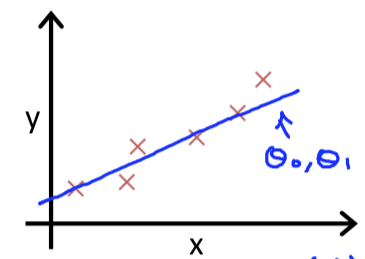
\includegraphics[width=0.7\textwidth, height=60mm]{example-graph.png}
                \\ \hline
                - must be linear relationship between independent and dependent variables \\
                - can be used with supervised learning \\ 
                - always seperates data with a straight line \\
            }
        \newline
        \newline
        \newline
    \end{minipage}
    
    \vspace{53.5pt}
    \fcolorbox{accent}{accent}{
    \begin{minipage}[t]{1\textwidth}
        \vspace{2pt}
        \center
        \textcolor{white}{\scriptsize \copyright 2018 - Machine Learning Collection 1/5 }
        \vspace{2pt}
    \end{minipage}
    }
\end{document}